\documentclass[a4paper]{article}
\usepackage{graphicx}
\usepackage{onecolceurws}
\usepackage{csquotes}
\usepackage{hyperref}
\usepackage{framed}
\usepackage{mdframed}
\usepackage{upquote}
\usepackage{lmodern}
\usepackage[normalem]{ulem}
\usepackage{caption}
\usepackage{subcaption}

\title{Sophize Markdown and Online Structured Data Extraction Tool }

\author{ Abhishek Chugh }

\institution{ Sophize Foundation\\ Bengaluru, India \\ abc@sophize.org }

\begin{document}
\maketitle

\newcommand\todo[1]{\textcolor{red}{TODO: #1}}


\begin{abstract}
Sophize is a novel mathematics library and discussion platform with a mission to help our users find and organize mathematical proofs. We have extended the Markdown language to represent the connections between mathematical objects that exist across various sources of knowledge. It allows embedding of semantic information (definitions, propositions and proofs) in documents. Using the new language, we showcase an interactive interface that helps users explore mathematics content on the web. We have also developed an online tool that helps in converting \LaTeX\space documents to this new language and adding semantic information.

\end{abstract}

\vskip 32pt

\section{Introduction}

\subsubsection*{Background: The Sophize Platform}

Sophize is a novel mathematics library and discussion platform. The author has developed the platform over the course of the last two years at \url{https://sophize.org}. Sophize's primary mission is to help users find existing proofs of mathematical statements, to discover new proofs, and to utilize this knowledge in their work. We combine knowledge from multiple resources and have accumulated thousands of definitions, theorems, and proofs from a wide variety of sources, including some published research, the PlanetMath encyclopedia, Wikipedia, and the Metamath formal system \cite{metamath}.

\subsubsection*{Proofs in Sophize}

Mathematical proofs are based on a variety of foundations such as ZFC, intuitionistic logic, and type theory. The arguments used in any proof are considered valid or not based on criteria that can vary. Most academic mathematics is peer-reviewed and published, but some mathematical proofs can be found in community curated sources such as Wikipedia. Proofs can also be algorithmically generated, and at the highest level of verification, they are represented and verified using a formal system. 

Sophize combines such an expansive range of proofs into a dense graph of propositions and logical arguments that aggregates knowledge from several documents and other data sources. We use this graph and combine it with the set of foundations and verifications chosen by each user to create proofs tailored to their needs. This introductory video gives an overview of the platform's offerings: \url{https://youtu.be/Wb1JbW9Otek}.

\begin{figure}[ht]
\begin{center}
\fbox{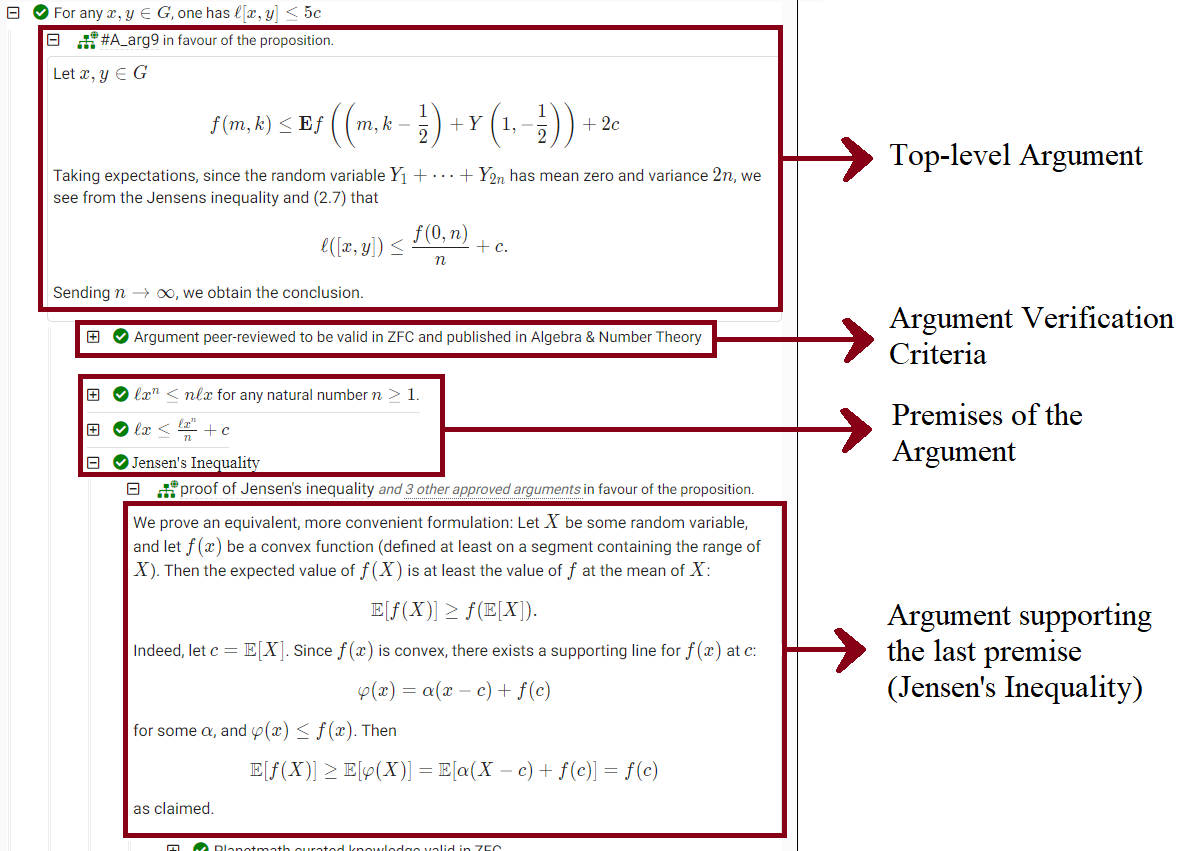
\includegraphics[height=12cm]{proof_tree}}
\caption{A proof displayed as a graph (tree) of arguments and propositions on the Sophize platform.}
\label{proof_tree}
\end{center}
\end{figure}

This work can also be seen as a step towards formalizing the network of information that exists in the connections of mathematical objects. The committee on planning a global library of the mathematical sciences recognized that this network is largely unexplored, and formalizing it has tremendous potential to accelerate math research \cite{sciences2014developing}.

Hence, we required novel knowledge organization techniques to connect mathematical entities from such a wide range of formal and informal knowledge sources. And thus, one of the main challenges towards building the Sophize platform was to create a simple way to embed mathematical entities on the web. This is the primary problem that this work addresses.

\subsubsection*{Contribution}

In this paper, we present the features of Sophize Markdown, an extension of the Markdown language. It is convenient enough to be used for casual discussions of mathematical ideas over the web. It is also powerful enough to embed mathematical entities such as definitions, theorems, and proofs from various sources, including formal systems. It thus plays an integral role in the two problems that we have mentioned above.

We have also developed an online tool that helps in extracting definitions, propositions and proofs from existing documents. It also allows users to easily add semantic information to documents.

Section 3 presents Sophize Markdown as a lightweight interface for representing math content, and Section 4 describes the online tool that help to easily add links and extract structured data from from existing documents. Finally, Section 5 concludes the paper.


\subsection*{Acknowledgements}
This work was supported by the International Mathematical Union and its Committee on Electronic Information and Communication. The author would like to thank Patrick Ion and Michael Kohlhase for their help in organizing our ideas and structuring the content of the paper.

\section{Preliminaries}

\subsection{Sophize's Data Model}
\paragraph{Before we describe the Sophize Markdown language, it will be necessary to briefly describe how Sophize models mathematical entities. The data model is published in JSON schema \cite{sophize_datamodel} and popular package managers such as MVN, npm and PyPI. We describe relevant parts of the concepts used here.}

\paragraph{A \textbf{resource} is an abstract concept inherited by all other top-level concepts like terms, propositions, and arguments. Each resource has a URI and contains fields such as search tags and citations.}

A \textbf{URI} consists of two parts: a namespace-like identifier called its dataset-id, which indicates the data source, and a resource-id that specifies the resource type and its unique name in the data source. The dataset-id may be omitted if it can be inferred from the surrounding context.

For example, the Pythagorean theorem (a \textbf{P}roposition) represented in the Metamath project may have the URI \emph{metamath/\textbf{P}\_pythagorean} and the definition of cone (a \textbf{T}erm) extracted from Wikipedia may have the URI \emph{wiki/\textbf{T}\_cone}. When used inside another resource in the `wiki' dataset, cone's definition can be referred to simply as \emph{T\_cone}.

\paragraph{A \textbf{term} is a clearly defined entity that can be used to make up a valid proposition. It can be a mathematical object, operator, symbol, data structure, algorithm, or even a person. `Meaningless' primitives in formal theories are also categorized as terms.}

\paragraph{A \textbf{proposition} is a grammatically valid statement that can be either true or false. Axioms, theorems, conjectures, hypotheses, lemmas, corollaries, and converses are all classified as propositions.}

\paragraph{An \textbf{argument} is a set of propositions called premises along with a concluding proposition that is claimed to follow from the premises. In addition, most arguments include supporting text that explains how the conclusion follows from the premises. A proof is seen as a directed graph of arguments and propositions.}

\section{Sophize Markdown}

Markdown is a lightweight markup language for creating formatted text using a plain-text editor. Markdown is very widely adopted on the web, and it makes it quite simple to add lists, headers, bold or italic fonts, images, and more. One can choose from several slightly varying Markdown specifications. We start with the widely supported CommonMark specification and create extensions for the features that we need. The extensions are implemented using the `markdown-it' \cite{markdown_it} JavaScript parser. The parser for Sophize Markdown produces an abstract syntax tree (AST). A separate renderer module utilizes the AST tree to create the appropriate HTML or Single Page Application (SPA) libraries. Many of the features of Sophize Markdown are demonstrated at: \url{https://youtu.be/5UYOpQwcjCk}

\subsection{Embedding structured data}  \label{structuredData}

With Sophize Markdown we can easily embed resources such as terms, propositions, and arguments. Links can be added using the resource's URI, and the following formats are supported:


\begin{itemize}

	\item \#URI[ $\vert$ OPTIONS ]

	Examples: \#wiki/T\_cone, \#planetmath/P\_covering\_lemma$\vert$NO\_LINK$\vert$LC

	\item \#(URI, \textquotesingle Custom\ Text\textquotesingle [ $\vert$ OPTIONS ])

	Examples: \#(wiki/T\_cone, \textquotesingle cones\textquotesingle), \#(P\_green\_tao\_theorem, 'Green–Tao Theorem'$\vert$NAV\_LINK)

\end{itemize}

There are multiple resource link options to embed a resource in the Markdown. These are required to make it convenient for the content creators to provide a rich experience to their readers. Some of the commonly used options are summarized below.

\subsubsection{Link Text Options}

\paragraph{\textbf{NAME} (default): This option fetches the resource and sets the link text to the name of the resource. For terms, the link text is set to the phrase of the term.}

\paragraph{\textbf{LOWER\_CASE (LC) or UPPER\_CASE (UC)}: These options become quite useful when adding a link in the beginning or middle of a sentence where adding the name in its default case would be grammatically incorrect.}

\paragraph{\textbf{Custom text}: A link can also explicitly specify the link text by enclosing it in single quotes.}

The following example shows the above options in use. Note that we assume that the dataset-id of URIs is available from the context and thus not specified in the URIs.

\begin{verbatim}
#P_cosine_law|UC is a generalization of the #P_pythagorean for all kinds of
#(T_triangle, 'triangles').
\end{verbatim}

\paragraph{The above code is rendered as:}
\begin{mdframed}
\dashuline{Law of cosines} is a generalization of the \dashuline{Pythagorean theorem} for all kinds of \dashuline{triangles}.
\end{mdframed}

\subsubsection{Link Type Options}

\paragraph{\textbf{OVERLAY\_LINK} (default): By default, clicking on links opens up a modal dialog with the resource's summary.}

\paragraph{\textbf{NAV\_LINK}: We can create a hyperlink to the resource's URL using the using NAV\_LINK option.}

\paragraph{\textbf{NO\_LINK}: NO\_LINK creates a non-clickable element whose hover text is the URI of the resource.}


For example, the following Markdown code has all three link types:
\begin{verbatim}
#T_matrix_multiplication|NO_LINK is a #(T_commutative_property, 
'non-commutative'|NAV_LINK) #T_binary_operation.
\end{verbatim}

\paragraph{The above code is rendered as:}
\begin{mdframed}
Matrix multiplication is a \underline{non-commutative} \dashuline{binary operation.}
\end{mdframed}
The first element shows `\#wiki/T\_matrix\_multiplication' on mouse-hover. The second link navigates the page to a different URL. Clicking on the third link pops up a modal dialog box like so:

\begin{figure}[ht]
\begin{center}
\fbox{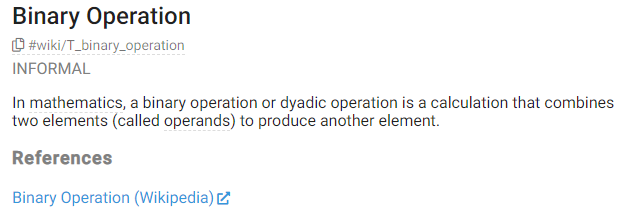
\includegraphics[height=5cm]{modal}}
\caption{Modal dialog box for the term binary operation. These boxes can also have content that uses all three types of links. }
\label{modal}
\end{center}
\end{figure}

\subsubsection{Resource Expansion}

Instead of creating a link, this option expands the resource in place. For terms and propositions, the definition and the statement are added in place, respectively. For arguments, its premises, conclusion, and the argument text is added.

The following is a sample article where we re-use concepts and theorems already extracted from multiple sources (say, Wikipedia and the Oxford dictionary):

\begin{verbatim}
# Conic section

A conic section (or simply conic) is a curve obtained as the intersection of the
#(wiki/T_conical_surface, 'surface') of a #wiki/T_cone with a #wiki/T_plane. There are
three types of conic sections.

## Ellipse
#oxford/T_ellipse|EXPAND #wiki/P_ellipse_area|EXPAND

## Parabola
#oxford/T_parabola|EXPAND The area of a parabola is unbounded.
...
\end{verbatim}

\paragraph{The above code is rendered as:}
\begin{mdframed}
\section*{Conic Section}
A conic section (or simply conic) is a curve obtained as the intersection of the \dashuline{surface} of a \dashuline{cone} with a \dashuline{plane}. There are three types of conic sections.

\subsection*{Ellipse}
An ellipse is a regular \dashuline{oval} shape, traced by a point moving in a plane so that the sum of its distances from two other points (the foci) is constant, or resulting when a cone is cut by an oblique plane which does not intersect the base.  The area $A_{ellipse}$ enclosed by an ellipse is $$A_{ellipse} = \pi a b$$where $a$ and $b$ are the lengths of the \dashuline{semi-major} and \dashuline{semi-minor} axes, respectively.

\subsection*{Parabola}
A parabola is a \dashuline{symmetrical} open plane curve formed by the intersection of a cone with a plane parallel to its side. The area of a parabola is unbounded.

...

\end{mdframed}

\subsubsection{Status Indicators}

For propositions, a Truth Value Icon indicating whether or not there is a proof is added next to the link. Clicking on the icon brings up the proof graph as shown in Figure \ref{proof_tree}. Similarly, an icon is added next to an argument which indicates whether the argument is valid or not. These options can be turned on or off depending on the input and the context. Further details require an in-depth understanding of the Sophize knowledge organization scheme which is not our focus here.

\subsection{Formal Language Support}

In formal languages, definitions of terms, statements of propositions, and supporting argument text may be parseable by an external parser. We can convert the externally parsed output into Markdown in such a case, where each term is automatically linked to the appropriate resource. This provides a convenient interface, where the user types in the native language, and the final output automatically allows users to explore all concepts that make up the input statement in depth. Currently, this is demonstrated in the use of Sophize Markdown with the Metamath language.

\begin{figure}[ht]
\begin{center}
\fbox{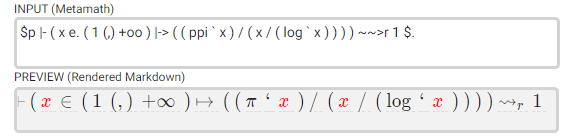
\includegraphics[height=3cm]{formal}}
\caption{The prime number theorem written in Metamath language and rendered as Markdown in real time.}
\label{formal}
\end{center}
\end{figure}

\subsection{\LaTeX\space Support}

While multiple applications extend Markdown to support TeX, there is no standardized syntax specification. However, Pandoc is the most widely used tool for converting \LaTeX\space to Markdown, and its specification is well documented and tested. Thus, we use their specification for our extension \cite{pandoc}:

\blockquote{Anything between two \$ characters will be treated as TeX math. The opening \$ must have a non-space character immediately to its right, while the closing \$ must have a non-space character immediately to its left, and must not be followed immediately by a digit. Thus, \$20,000 and \$30,000 won’t parse as math. If for some reason you need to enclose text in literal \$ characters, backslash-escape them and they won’t be treated as math delimiters.

For display math, use \$\$ delimiters. (In this case, the delimiters may be separated from the formula by whitespace. However, there can be no blank lines between the opening and closing \$\$ delimiters.)}

The following example summarizes the specification:
\begin{quote}
\begin{verbatim} 
Einstein's most famous equation is $E=mc^2$ but it is his handwritten theory of 
happiness is what fetched $1.3 million recently. While it may not fetch many \$s, I 
like the field equations more: $$G_{\mu \nu }+\Lambda g_{\mu \nu }=\kappa T_{\mu \nu }$$
\end{verbatim}
\end{quote}


The above Markdown code is rendered as:
\begin{mdframed}
Einstein's most famous equation is $E=mc^2$ but it is his handwritten theory of happiness is
what fetched \$1.3 million recently. While it may not fetch many \$s, I like the field
equations more: $$G_{\mu \nu }+\Lambda g_{\mu \nu }=\kappa T_{\mu \nu }$$
\end{mdframed}

\section{Online Structured Data Extraction Tool}

The online tool developed as a part of this project provides two functionalities to users. Firstly, it allows Sophize library maintainers to easily select and extract semantic knowledge (definitions, propositions and proofs) from documents using an web-based interactive interface. Secondly, it makes it easy to add resource links (See Section \ref{structuredData}) to markdown documents.

The major components of the tool are described in the following sections.

\begin{figure}[ht]
\begin{center}
\fbox{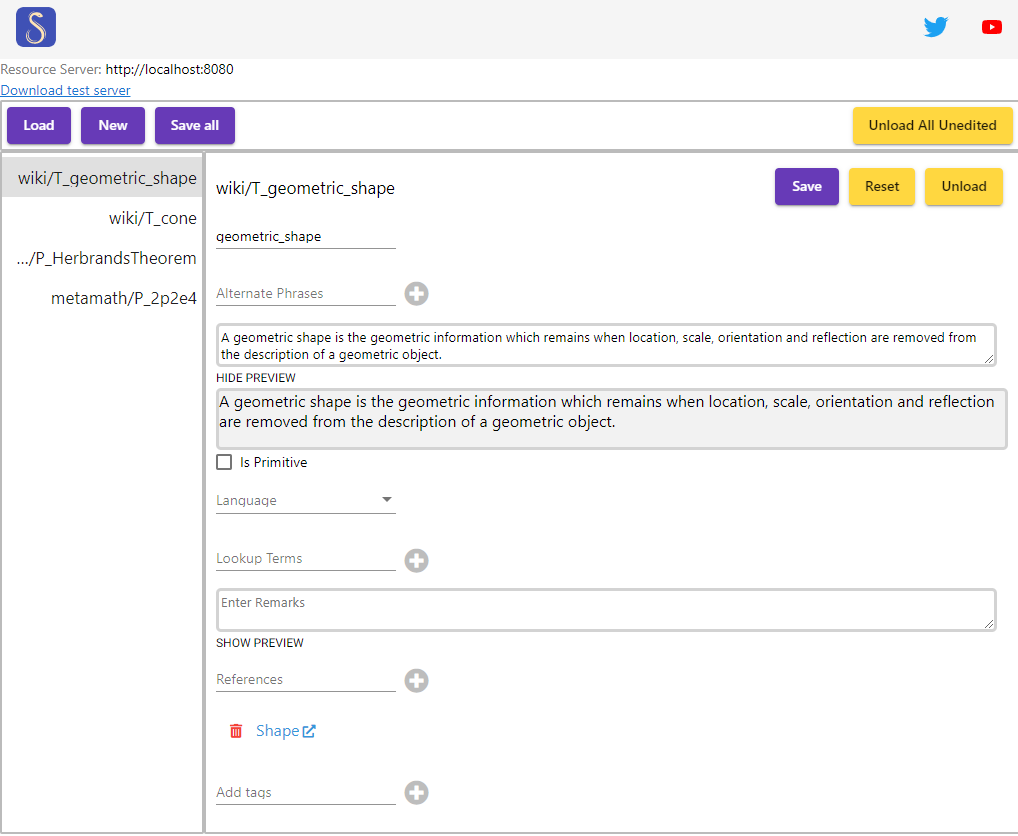
\includegraphics[height=12cm]{sdet_overview}}
\caption{Main page of Structured data extraction tool.}
\end{center}
\end{figure}

\subsection{Managing Resources}

The tool has been designed to allow multiple resources to be modified simultaneously. The tool reads and writes multiple resources to an external server. Any external server that implements these two APIs (read and write) can be used with this tool. Such a server could store these resources in any kind of database. As a part of this project, we also provide a simple server that manages resources by writing and reading resources to and from the local disk.

The tool loads resources from the external server in the local storage section of the browser. This allows the modifications to persist even the page is closed or refreshed. Any new resources created or extracted are also placed in local storage. The user can modify all resources simultaneously and once the required changes are made, the resources are written back the external server with a single click.

\subsection{Webpage for extracting/embedding structured data}
For ease of use, all the features of the tool have been integrated into a single page. The top section of the page has buttons for loading, unloading, saving, and creating new resources. The left navigation bar lets users easily switch between different resources currently loaded. Any changes made are automatically written to the browser's local storage before the user chooses to save their changes to the external server.

In addition, a new context menu shows up when the user has selected a portion of text in any of the resource fields. The context menu has options to extract the selected text as a definition, proposition, or argument and to convert the selected text to a Sophize Markdown link. Thus, by simply selecting and right-clicking the text we can perform the task of embedding and extracting semantic data in documents. The various options of these tasks are displayed using convenient modal dialogs.


\begin{figure}[ht]
\begin{center}
\begin{subfigure}{.5\textwidth}
  \centering
  \fbox{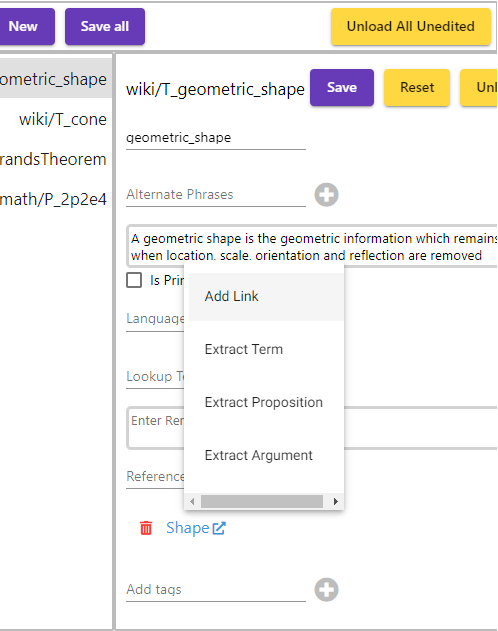
\includegraphics[width=0.74\linewidth]{sdet_contextmenu}}
  \caption{Context menu to add link and extract resources}
  \label{fig:sub1}
\end{subfigure}%
\begin{subfigure}{.5\textwidth}
  \centering
  \fbox{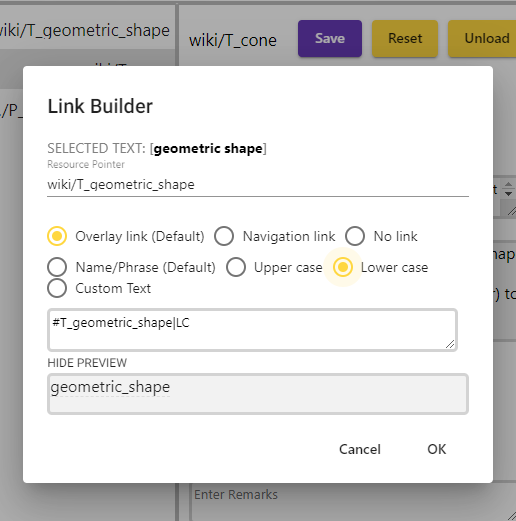
\includegraphics[width=0.93\linewidth]{sdet_add_link}}
  \caption{Adding Sophize Markdown Link}
  \label{fig:sub2}
\end{subfigure}
\caption{Select and right-click interface for embedding and extracting structured data.}
\end{center}
\end{figure}

\subsection{Server to convert \LaTeX\space document to Markdown }

Since most mathematical knowledge is present in \LaTeX\space documents, there is a need for an easy way to first convert these documents to Markdown before this tool can be used on them. Pandoc is the obvious choice for this conversion. A Python server that utilizes the Pandoc converter has been developed. It also performs input and output processing to circumvent some limitations of the Katex library that is used for rendering Math mode content. Using this server we provide a convenient copy-paste interface in the tool for easy conversion.


\section{Conclusion and Future Work}

We have presented Sophize Markdown, a lightweight language for representing mathematical knowledge on the web. Using this language, we can easily embed mathematical entities like definitions, theorems, and proofs, making it very convenient to find and browse relevant content. Sophize Markdown plays a central role in organizing proofs from various data sources on the Sophize platform. While there are other ways to represent semantic knowledge, such as content MathML and OpenMath, their scope is somewhat limited to specifying the meaning of the mathematical formula. The sTeX system \cite{Kohlhase2008} is perhaps most similar to Sophize Markdown but it needs creation of \LaTeX\space documents and use of \LaTeX ML systems. This makes its use in real-time web workflows impractical.

In the future, we want to make a substantial portion of math literature embedded with structured data available at a much greater scale. Thus, we will improve Sophize Markdown's support for \LaTeX\space features like equation numbering, tables, and references. We also need to improve rendering time for large documents. In addition, we will be improving the tool to significantly reduce the manual effort required to extract resources and add links by creating better interfaces and automating some tedious tasks.This process will also be aided by the recent supervised learning techniques \cite{ginev2019scientific} that classify scientific statements in literature.


\subsection*{Sources}
All code for this project has been released under the MIT license. The Sophize Markdown parser and its Angular renderer source code are available at \url{https://github.com/Sophize/sophize-md-parser} and \url{https://github.com/Sophize/ngx-sophize-md-renderer}, respectively. The NPM packages for these projects are named `sophize-md-parser' and `ngx-sophize-md-renderer'.

The source code for Structure Data Extraction Tool is available at \url{https://github.com/Sophize/structured-data-extractor} and it is hosted at \url{https://sdet.sophize.org}. The code for the server that converts \LaTeX\space documents to Markdown is at \url{https://github.com/Sophize/md-convert-server}.

\bibliographystyle{alpha} 

\bibliography{mybib}

\end{document}
